\noindent Dear airline executive:

	We are the \defword{IMMC Mathematical Modeling Group}. We've heard that you have problem on saving time and raising efficiency of boarding and disembarking. In our opinion, this may be caused by the inefficiency of the boarding and disembarking plan you have used. It gives us great pleasure to give some suggestions to you  about these two process based on our model.

	To begin with, we want to talk about boarding. whatever kind of strategy your company adopts, it's crucial that the features below are taken into account:

	\begin{itemize}
		\itembf{Stability.}

		While minimizing total boarding time, the model itself must be solid enough, or in other words, the strategy itself should not change while the relative parameters of passengers change. (For example, even when some passengers bring more luggage with them, it's important to keep the model as it originally was.) The more structured your boarding strategy is, the less an impact will variations in these passenger-based parameters have on the overall time of boarding.
		\itembf{Hommization.}

		Firstly, try a boarding way that minimizes the time a passenger offers his/her seat, and thus lowering anxiety and annoyance of unnecessary seat-offering. Therefore, it's crucial to make sure that the overall boarding process generally lets passengers near the window board first, and lets those next to the aisle board last. As a result, passengers can get seated with satisfaction and pleasantly start the journey.

  		Secondly, make sure that families or friends board in succession. To be more specific, please first check whether passengers in the same line are put together, as passengers familiar with one another tend to choose adjacent seats. What's more, families with the young should righteously board together.
		\itembf{Efficiency.}

		Nobody likes being stuck in a queue for too long. Therefore, with stability and hommization taken into consideration, please choose the option with the least queuing time (also equivalent to the least overall boarding time). For instance, under the single-aisle scenario, front-to-back boarding is catastrophic, since each person stowing his/her luggage causes a 'fullstop', with latter passengers not even on the plane, and therefore can do nothing but wait.

		And with these three factors combined, we get a solution! We call it 'Back to front, section by section, and window middle aisle'.

		Before boarding, each passenger should first get a 'boarding' number. We suggest the plane be divided into three sections, with boarding sequence from back to front (boarding number 1, 2, and 3). For each group of passengers with the same boarding number, group them by row, also back to front, so that more passengers can board at the same time. The following diagram gives the optimal strategy:
		\begin{center}
			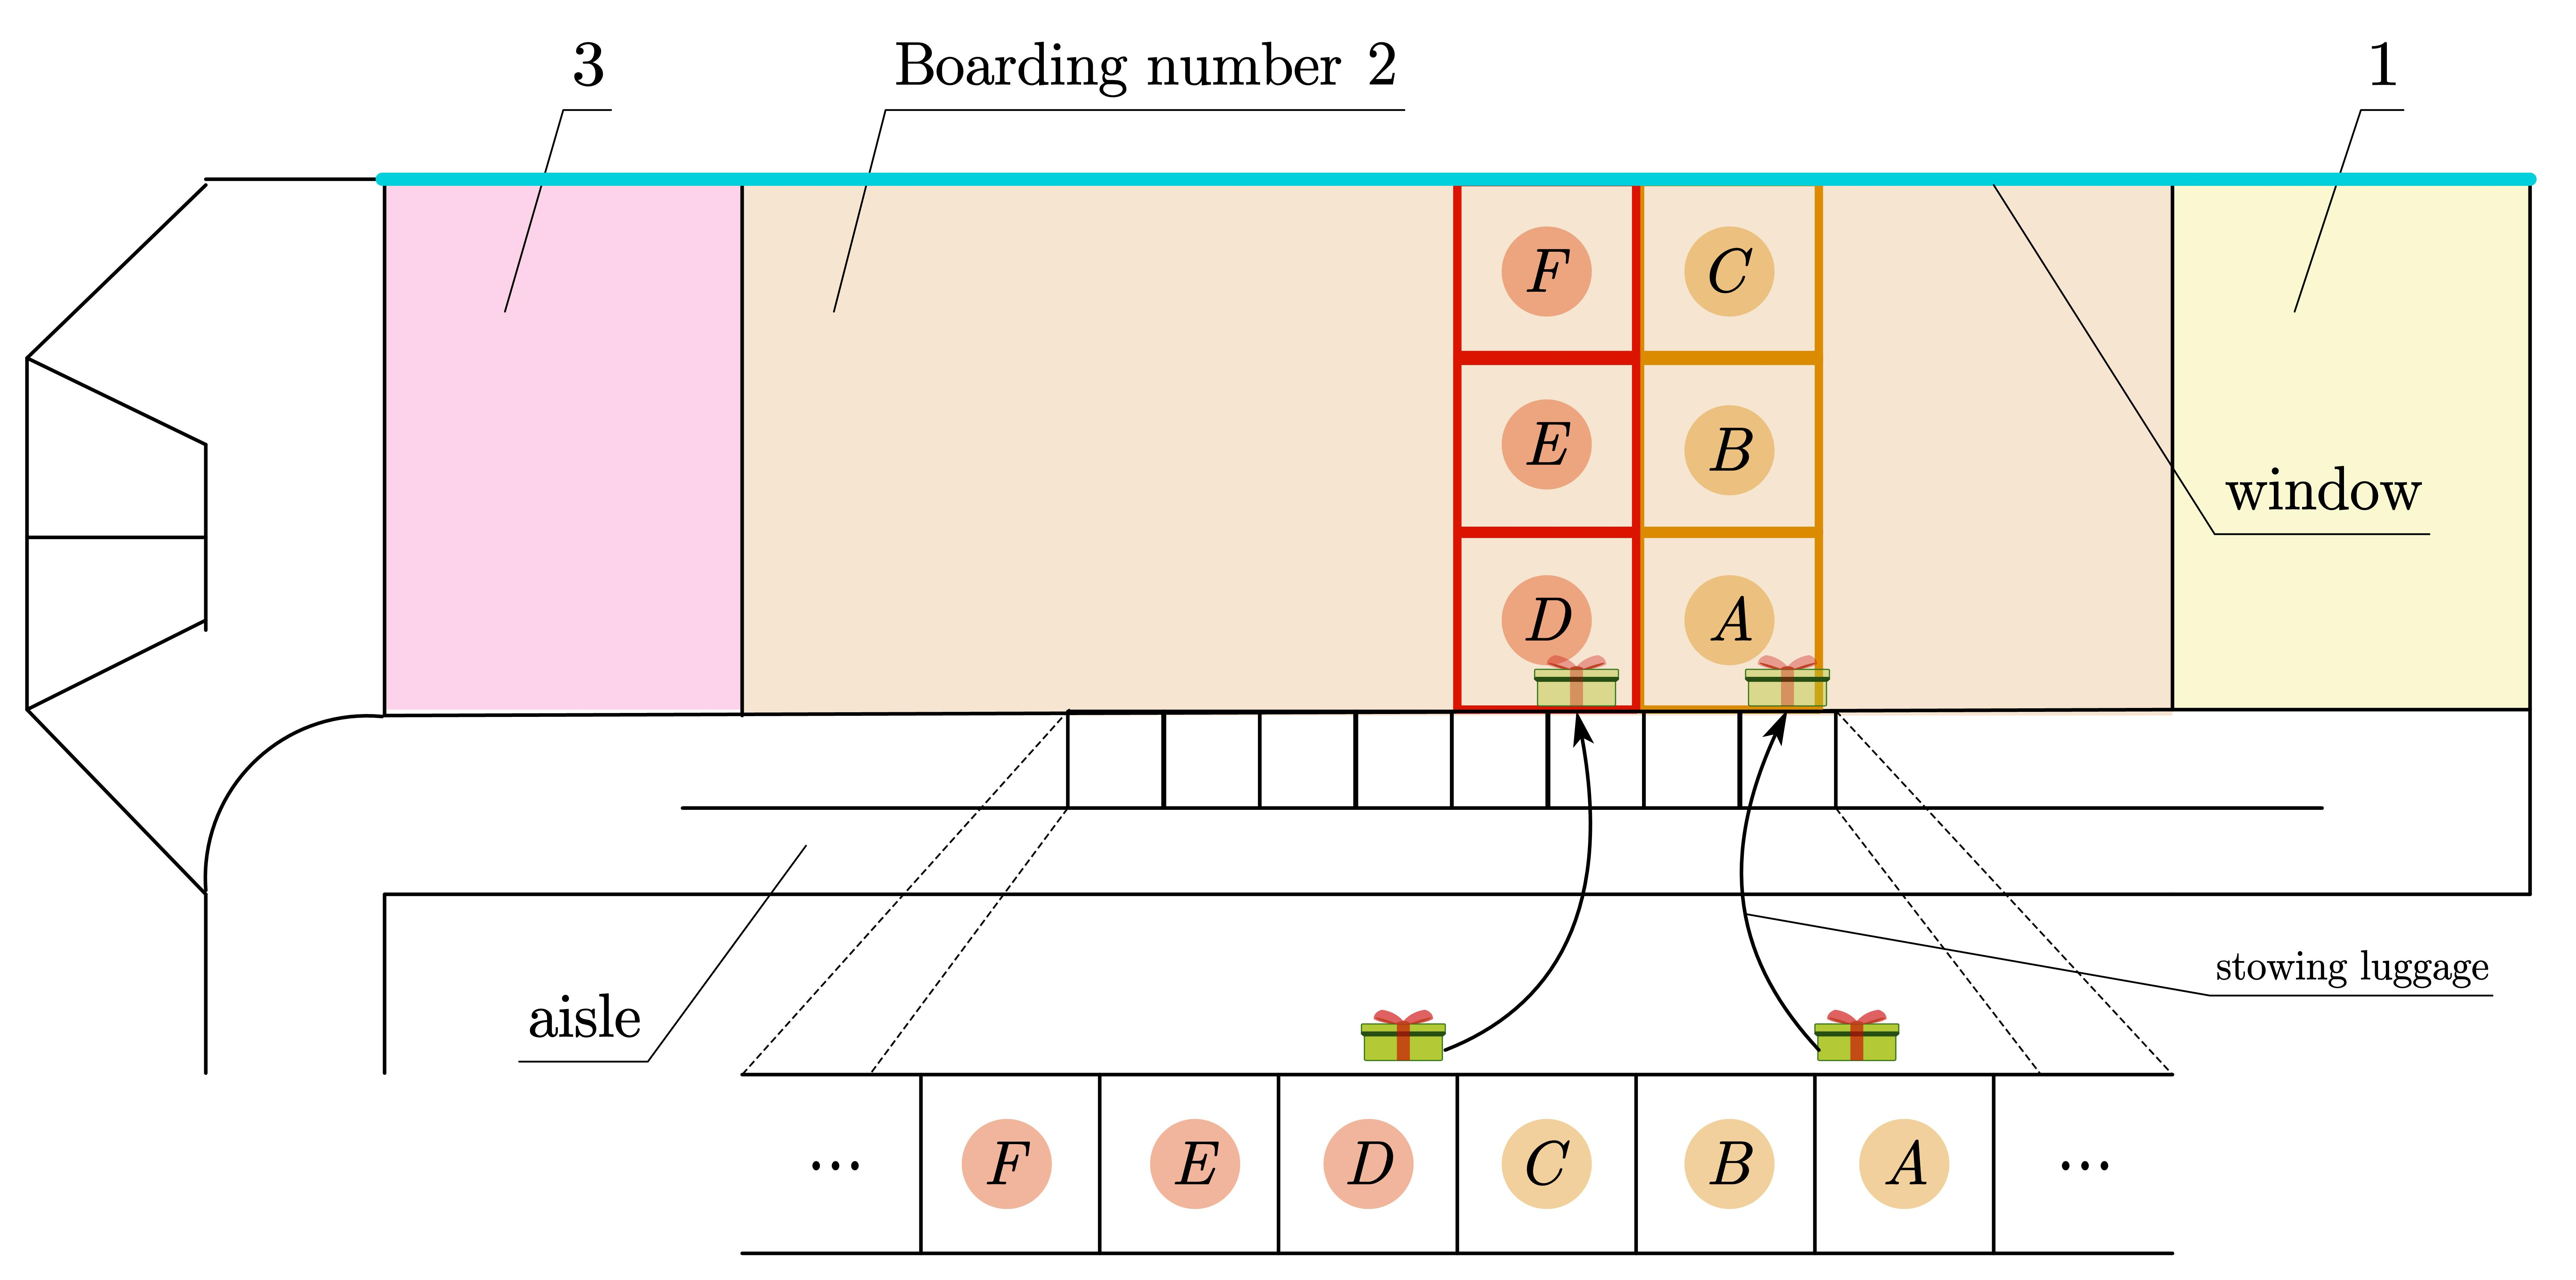
\includegraphics[width=11.6cm]{advice-ver2.jpg}
		\end{center}
	\end{itemize}

	Also, here are some small tips we've concluded from our model:
	\begin{enumerate}
		\itembf{If there are several aisles in your plane, avoid blocks in general aisles.}

		General aisles are especially important in the whole boarding process. It actually controls other branch aisles. If too much people in the general blocks the way, it may lead to a thorough collapse of this process. Therefore, you must make sure the general aisles are blocked.
		\itembf{Divide the plane into several sections.}

		If your plane map is especially complicated, don't worry about it! Divide the whole plane into several parts according too it's geometric shape and find out the best strategy seperately based on the suggestions we've given above. Later, combine them all together and implement them seperately.
		\itembf{Provide enough space  for luggages.}

		Nowadays, to save cost on consignment, many passengers may choose to bring their luggages with them to the plane. If there isn't enough place for luggages, passengers may spend more time on dealing with their luggages. This means more time for others in waiting, which will lead to an increase in the total boarding time (caused by queuing) and a rise in passengers' negative emotions.

		\itembf{Prevent queue-jumping.}

		For structured boarding schemes such as the process introduced above, even a tiny portion of passengers who swap their sequences in the initial queue can have a dramatic effect on the overall boarding time. Therefore, passengers should strictly follow their boarding groups in advance to avoid such incidents.
	\end{enumerate}

	As for the disembarking part, our suggestion is that you needn't worry much about it. According to the result we've got, the best plan is actually let passengers get "stuck" in the aisle in order! Under this circumstance, all that you need to do is actually let the passengers bear their seat number in mind. Passengers first grab their bags, and get into the aisle from front to back, aisle to window, ensuring that lines are kept together and that the aisle is always full.

	Hope that our suggestions can help you, looking foward to your reply!

	\noindent Yours sincerely,

	\noindent \defword{IMMC Mathematical Modeling Group}